% !TEX root = ../thesis.tex


\chapter{Conclusion and Future Work}
\label{cha:dmd_future}
We presented an algorithm to iteratively correct for deviations in patterns produced from DMDs. To do this, we first developed a method to reliably calibrate a camera such that the camera pixel coordinates can be mapped to their corresponding DMD pixel counterparts. We can then correct for image deviations by using feedback from the captured intensity as well as by suppressing minima and maxima through the careful switching of select pixels on the DMD. 
We have shown that this algorithm can correct structures that are as little as \SI{3}{px} spaced apart on the camera. With intensity noise, fluctuations can be reduced to an RMS error below \SI{1}{\percent}. These results were achieved with pixel to pixel magnifications of \num{2.2} and \num{5}. This shows that even when the DMD is underresolved, corrections are still possible.

Although these are satisfying results, the algorithm is currently limited to linear effects where we assume that the DMD only influences the intensity on the camera in one specific region. However, due to interference effects, there might also be deviations caused by non-linear effects. In that case, even with a perfect pixel to pixel mapping from the camera to the DMD, we can not easily determine which pixels are affected by changes on the DMD. To solve this problem, a machine learning algorithm could analyse the output of several images and deduce the correct, even non-linear mapping based on these. 

For experiments where the highest possible accuracy is required, one could utilise two separate DMDs. One of them would provide the large scale pattern and the other could be used with a lower powered laser to provide corrections with the highest dynamic range that one DMD can use.

\pagebreak
\noindent Finally, I want to end this part with one last demonstration image that was created using the presented correction algorithm.

\begin{figure}[htbp]
    \captionsetup{list=no}
    \centering
    \pdfpxdimen=\dimexpr 1 in/96\relax
    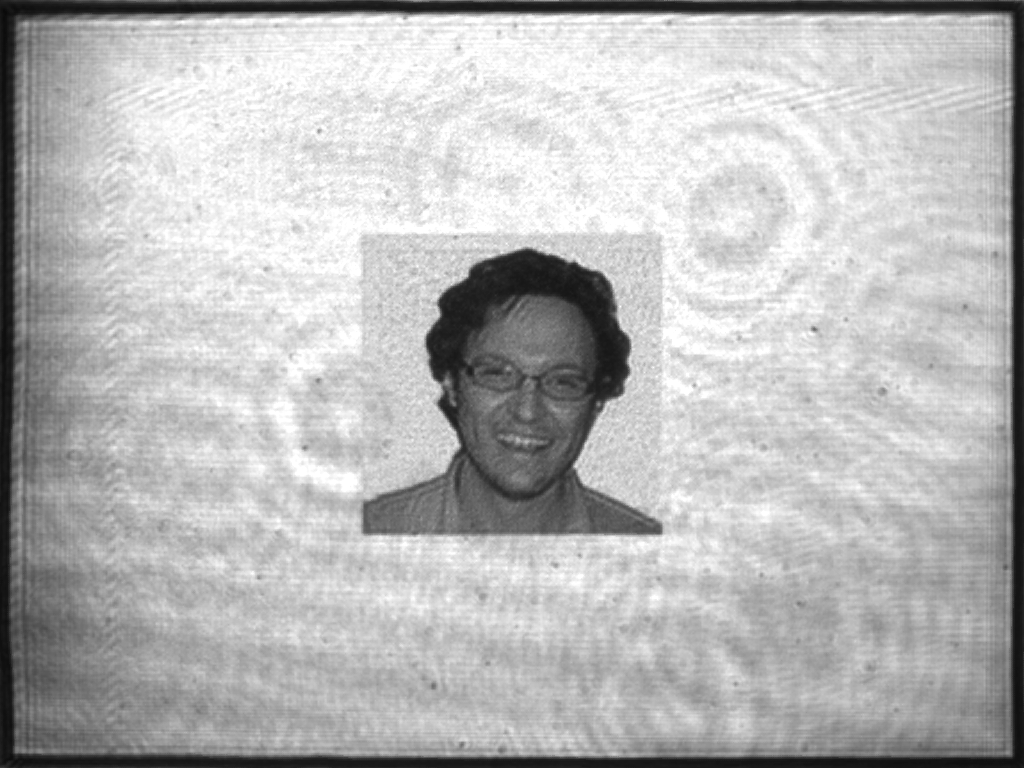
\includegraphics[trim=362px 234px 362px 234px,clip,width=.33\textwidth]{DMD/Zoran-Mask-result}
    \caption{Zoran}
    \label{fig:zoran}
\end{figure}
